\section{Vercel}
El despliegue de la aplicación se realiza utilizando Vercel, la plataforma de hosting creada por los mismos desarrolladores de Next.js. Esto proporciona una integración óptima y simplifica significativamente el proceso de despliegue, garantizando compatibilidad con el framework.

Vercel Inc., anteriormente conocida como ZEIT, es una empresa estadounidense de tecnología especializada en edge computing, alojamiento web y redes de entrega de contenido. La infraestructura de Vercel se apoya en servicios como Amazon Web Services y Cloudflare para garantizar un alto rendimiento y disponibilidad.

Vercel es una plataforma de hosting orientada a aplicaciones frontend y serverless. Se destaca por su facilidad de uso, optimización para Next.js y opciones avanzadas de despliegue continuo.

\section{Límites y características del plan Hobby en Vercel}

El plan gratuito \textit{Hobby} de Vercel ofrece una variedad de funcionalidades y límites que se ajustan a proyectos personales o de pequeña escala. A continuación, se describen las principales características agrupadas por categorías:

\subsection{Límites y características del plan Hobby}

\begin{table}[htbp]
    \centering
    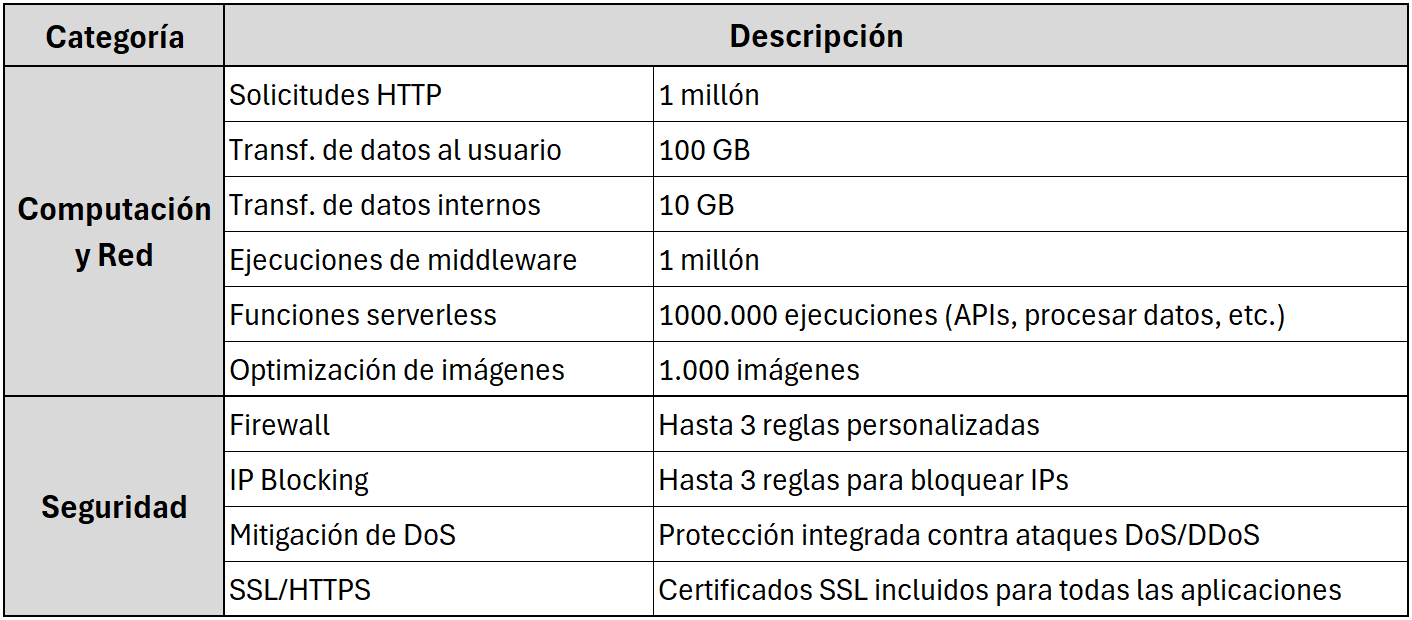
\includegraphics[width=0.9\textwidth]{figures/vercel_plan_hobby.png}
    \captionsetup{skip=10pt}
    \caption{Límites y características por mes del plan \textit{Hobby} de \textit{Vercel}.}
    \label{tab:vercel_plan_hobby}
\end{table}


\section{Proceso de Despliegue}
La integración con Vercel permite realizar despliegues de manera sencilla. La plataforma está conectada con GitHub, lo que permite desplegar la aplicación automáticamente cada vez que se realiza un \textit{push} a la rama principal.

Además, Vercel proporciona vistas previas para \textit{pull requests} o ramas distintas a la principal, lo que facilita la revisión de cambios antes de publicarlos en producción.

\subsection{Configuración de Variables de Entorno}
Para el correcto funcionamiento de la aplicación, es necesario configurar variables de entorno en el panel de control de Vercel. Estas incluyen credenciales de la API de Spotify y el dominio del despliegue para que los \texttt{fetch()} internos funcionen correctamente. Se debe evitar codificar directamente las URLs en el código y en su lugar utilizar variables de entorno, asegurando flexibilidad y seguridad.

\subsection{Análisis y Monitoreo en el Dashboard de Vercel}
Vercel ofrece un panel de control desde donde se pueden visualizar diversas métricas y opciones de configuración, entre las que se incluyen:
\begin{itemize}
    \item Estado de los despliegues y logs en tiempo real.
    \item Historial de versiones desplegadas.
    \item Estadísticas de tráfico y rendimiento.
    \item Configuración de dominios y DNS.
\end{itemize}

\section{Ejecución Automática de Tests}
Una funcionalidad deseable en el despliegue es la ejecución automática de tests para garantizar que cada nueva versión sea estable antes de llegar a producción. Hay dos enfoques posibles:
\begin{enumerate}
    \item Configurar GitHub Actions para ejecutar los tests antes de desplegar.
    \item Configurar Vercel para ejecutar tests en cada despliegue.
\end{enumerate}
Actualmente, se está evaluando cuál de estas opciones implementar. Una posible estrategia es usar GitHub Actions para correr los tests unitarios y de integración antes de hacer el \textit{push} a la rama principal.
